\documentclass[conference]{IEEEtran}
\IEEEoverridecommandlockouts
% The preceding line is only needed to identify funding in the first footnote. If that is unneeded, please comment it out.
\usepackage{cite}
\usepackage{amsmath,amssymb,amsfonts}
\usepackage{algorithmic}
\usepackage{graphicx}
\usepackage{textcomp}
\usepackage{xcolor}
\def\BibTeX{{\rm B\kern-.05em{\sc i\kern-.025em b}\kern-.08em
    T\kern-.1667em\lower.7ex\hbox{E}\kern-.125emX}}
\begin{document}

\title{People Behavior Tracking (PBT)\\}

\author{
Hernán Contigiani\textsuperscript{\dag}\textsuperscript{1}, Pasquinell Urbani*\textsuperscript{2} \\
\textsuperscript{\dag}\textit{Facultad de Ingeniería - Universidad de Buenos Aires (FI-UBA)} \\
\textit{Universidad Tecnológica Nacional (UTN)} \\
\textsuperscript{1}\small hernan4790@gmail.com \\
\normalsize *\textit{Universidad de Chile (UCh)} \\
\textsuperscript{1}\small purbanir@gmail.com
}
\maketitle

\begin{abstract}
El presente documento describe el diseño de un sistema de monitoreo de personas. El sistema permite monitorear mediante técnicas de inteligencia artificial basadas en visión por computadora los desplazamientos que realiza una persona en un espacio y obtener métricas de las zonas que visitó. Se presentan los resultados y mejoras de la arquitectura propuesta respecto a las soluciones que se pueden hallar en la bibliografía, y cómo esta propuesta de trabajo se transformó en una solución real llevada a cabo en conjunto con la empresa Globant S.A.
\end{abstract}

\begin{IEEEkeywords}
seguimiento de personas, aprendizaje profundo, re-identificación de objetos
\end{IEEEkeywords}

\section{Introducción}
El propósito de este trabajo fue el desarrollo de un sistema de monitoreo de personas. Tiene como principal objetivo estudiar los movimientos que realiza un individuo al ingresar y transitar un espacio a fin de obtener métricas sobre las zonas que visitó. Para cumplir este objetivo es necesario poder detectar a las personas que aparecen en el video tomado por una cámara, realizar el seguimiento de cada una e identificarlas aún cuando desaparecen del espacio de visión por unos minutos. La solución debe ser capaz de realizar el seguimiento en espacios muy transitados, como puede ser una tienda, un negocio o un supermecado.

Existen distintas soluciones abiertas basada en inteligencia artificial que resuelven parte de este problema, tanto en librerías de visión por computadora como OpenCV \cite{b1}, proveedores de \textit{hardware} como NVIDIA \cite{b2} o Intel \cite{b3} y en proveedores de soluciones \textit{cloud} como Amazon \cite{b4}  o Google \cite{b5}. Los algoritmos y modelos que pueden utilizarse de estos proveedores para el seguimiento de personas carecen de robustez por sí solos, dado que solo funcionan en espacios abiertos libres de obstáculos o en donde la densidad de personas en el espacio es baja. Mantener a cada persona correctamente identificada sin perderla o confundirla (mantener el identificador único de seguimiento, su ID) es muy complejo, debido que las personas en movimiento forman y disuelven grupos, cambian su pose constantemente, pueden salir y volver de escena, etc. Este trabajo aborda esta problemática.

\section{Sistema de seguimiento de personas}

\subsection{Tecnologías empleadas}

Para desarrollar el sistema de seguimiento se emplearon técnicas de visión por computadora \textit{(computer vision)} \cite{b6} del campo del aprendizaje profundo \textit{(Deep Learning)} \cite{b7} entre las cuales se encuentran:
\begin{itemize}
\item Detección de objetos: técnica que permite detectar múltiples objetos \cite{b8} (personas, vehículos, animales, etc) en una imagen indicando la ubicación de cada objeto y el tipo de objeto detectado. Las detecciones son representadas con una caja de detección \textit{(bboxe)} \cite{b9} , la cual posee las coordenadas en píxeles para ubicar al objeto en la imagen. En este trabajo se utilizó \textit{Yolo (You Only Look once)} \cite{b10} como modelo detector de objetos configurado para detectar personas en imágenes y conocer su ubicación.
\item Seguimiento de objetos: técnica que permite seguir múltiples objetos en imágenes \cite{b11} asignando a cada objeto un identificador único (ID) de seguimiento. Este identificador es un valor numérico incremental que permite distinguir de forma univoca a cada objeto encontrado en la imagen. Se espera que se mantenga el mismo número para el mismo objeto mientras este permanezca a la vista. En este trabajo se utilizó \textit{Deepsort (Deep Simple Online Tracking)} \cite{b12} el cual consume las detecciones (bboxes) del detector y asigna a cada objeto un ID único.
\item Extraer características visuales: técnica que permite extraer vectores de características de una imagen de una persona que la representan y diferencian de otra. El extractor toma las detecciones que arroja el detector y genera un vector numérico por cada persona que representa las características observadas en ella.  Las características que arroja el extractor son números, no representan ninguna cualidad física específica sino más bien un espacio numérico que la representa y diferencia de otras. En este trabajo se utilizó \textit{Osnet (Omni-Scale Network)} \cite{b13} como modelo extractor de características.
\end{itemize}

\subsection{Desafíos en el seguimiento de personas}

Los desafíos que se detallan a continuación son problemas que presentan en este tipo de sistemas de monitoreo a la hora de seguir un objeto con el mismo identificador:
\begin{itemize}
\item Pérdida del identificador de seguimiento (ID): ocurre cuando una persona pasa por detrás de otro objeto que la ocluye. El objeto que la ocluye puede ser estático (un mueble, un cartel, etc) o dinámico (otra persona o grupo de personas en la escena).
\item Intercambio de identificador de seguimiento (ID): ocurre cuando dos personas se cruzan en movimiento. Al momento que ambas personas se cruzan, sus bboxes poseen una ubicación geométrica y un vector de movimiento similar. Estos factores producen que el modelo seguidor no pueda diferenciar las detecciones, aumentando significativamente la probabilidad de que el modelo intercambie sus identificadores por error.
\end{itemize}

Estos desafíos son el principal problema de los sistemas que se mencionaron en la introducción, que se basan unicamente en modelos de detección y seguimiento de objetos. Estos sistemas requieren un ajuste fino de los parámetros de configuración de la cámara y del área de visión a fin de reducir los errores al mínimo \cite{b14}. En este trabajo se busca superar estos desafíos agregando a la ecuación un modelo de extracción de características y técnicas de re-identificación por aprendizaje automático.

\subsection{Métricas de evaluación del sistema}

Los sistemas de monitoreo o seguimientos de objetos se los evaluá según cuantos objetos pudo el sistema detectar y seguir correctamente. Para este trabajo se definieron los siguientes requerimientos de seguimiento:

\begin{itemize}
\item Se considerará que una persona es correctamente monitoreada si al menos se mantuvo su seguimiento el 80\% del tiempo que circuló en el
recinto.
\item Se considerará que el sistema funciona dentro de los parámetros aceptables si entre el 80\% y 100\% de las personas en el video fueron correctamente monitoreadas.
\end{itemize}

\section{Diseño e implementación}

\subsection{Arquitectura}

En la figura \ref{fig:esquemaGeneral} se observa un diagrama general de la solución y las etapas que la componen:

\begin{figure}[htbp]
\centerline{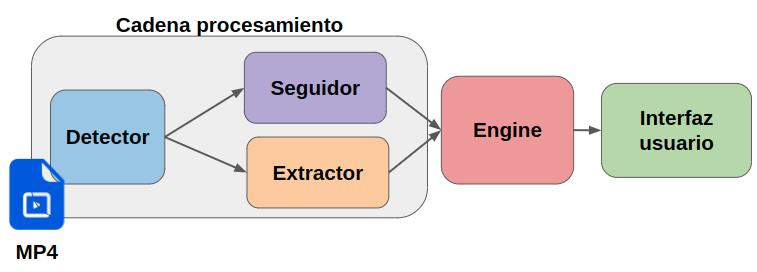
\includegraphics[scale=.4]{./Figures/esquemaGeneral.jpg}}
\caption{Diagrama general de la solución.}
\label{fig:esquemaGeneral}
\end{figure}

\begin{itemize}
\item Cadena de procesamiento: etapa compuesta por los tres modelos de inteligencia artificial (detector, seguidor, extractor). Cada modelo en la cadena realiza un aporte al sistema de detección y seguimiento de personas. El resultado de esta etapa son las detecciones y características de cada persona observada en el video suministrado al sistema.
\item Motor de seguimiento (Engine): etapa encargada de mejorar la precisión de seguimiento mediante re-identificación y manejo de oclusiones. Recibe los datos de la etapa de cadena de procesamiento y calcula las métricas de monitoreo que luego se presentan en la interfaz de usuario disponible en la aplicación web.
\item Interfaz de usuario: aplicación web que utiliza el usuario para configurar las zonas de interés en el recinto y observar la evolución de las métricas y el monitoreo de personas.
\end{itemize}

\subsection{Re-identificación}
\label{seccionreid}

El “Engine” utiliza los vectores de características de cada objeto para agrupar los datos \textit{(clustering)} que corresponden a una misma persona. Clustering es el proceso que permite establecer relaciones entre elementos que poseen características en común conformando grupos de datos \textit{(clusters)}. En la figura \ref{fig:clusterPersonas} se observa cómo las distintas capturas tomadas de una persona en diferentes ángulos se agrupan para formar un cluster.

\begin{figure}[htbp]
\centerline{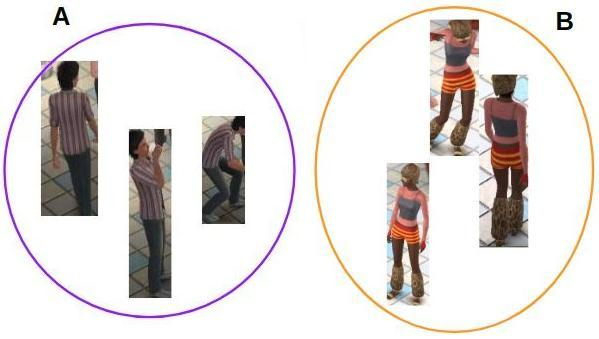
\includegraphics[scale=.5]{./Figures/clusterPersonas.jpg}}
\caption{Segmentación de personas en clusters.}
\label{fig:clusterPersonas}
\end{figure}

El proceso de re-identificación de personas busca relacionar una nueva persona por su vector de características con un cluster ya conformado. El objetivo es mantener el seguimiento de una persona con el mismo cluster, es decir con el mismo identificador, a pesar de que se haya salido de escena por unos segundos. Para
poder calcular la similitud entre el vector de una persona y los diferentes clusters se utiliza la similitud coseno \cite{b15}, que devuelve un valor entre -1 y 1 siendo 1 la expresión para máxima similitud.

Cuando el modelo seguidor pierde el identificador de seguimiento de una persona o se intercambia por uno erróneo, el “Engine” ejecuta el proceso re-identificación para asignar a esa persona su cluster correspondiente. El proceso de re-identificación está conformado por una serie de \textit{thresholds} y \textit{timers} a fin de evitar generar falsos positivos. Estos valores de configuración se obtuvieron de forma empírica utilizando videos de diferentes recintos y diferentes personas, analizando la calidad de los clusters en cada ensayo mediante una matriz de similitud \cite{b16}.

\section{Resultados}

\subsection{Ensayos}

Dado que para ensayar todas las condiciones se necesita involucrar varias personas a lo largo del video, se optó por utilizar el videojuego “Los Sims 3” \cite{b17}, en el cual es posible crear un ambiente totalmente a medida y personajes que interactúan en él. El juego permite crear personajes con diferentes personalidades por lo que cada uno interactúa de forma singular con el espacio pudiéndose obtener distintas métricas por el tiempo que se desee que dure el ensayo. En la figura \ref{fig:sims} se observa el entorno creado para ensayar el sistema.

\begin{figure}[htbp]
\centerline{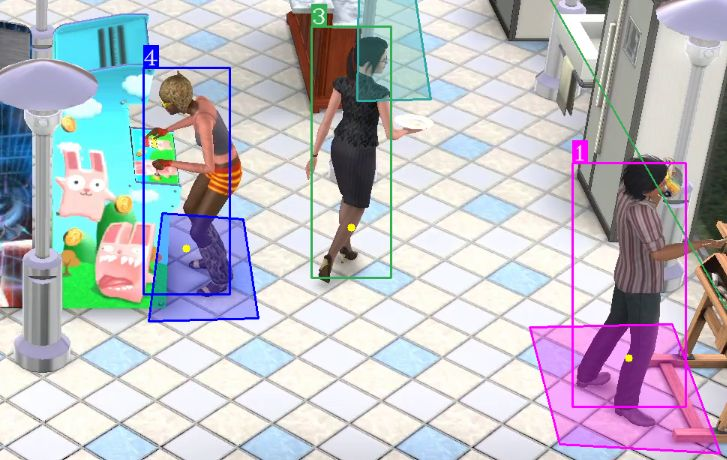
\includegraphics[scale=.30]{./Figures/sims.jpg}}
\caption{Escenario creado en el video juego ``Los Sims 3''.}
\label{fig:sims}
\end{figure}

El video generado a partir del simulador permitió ensayar y validar todas las funcionalidades del sistema. Se ensayaron tres sistemas diferentes a fin de comparar las técnicas incluidas en cada uno.

\begin{itemize}
\item Yolo y Deepsort: sistema basado unicamente en el detector Yolo y el seguidor Deepsort, tal cual se encuentra disponible en la web.
\item Engine10: sistema basado en el detector Yolo, el seguidor Deepsort y el postprocesado del Engine v1.0 utilizando los vectores de características para el manejo de oclusiones y re-identificación de personas.
\item Engine16: sistema basado en el detector Yolo, el seguidor Deepsort y el postprocesado del Engine v1.6 que incorpora la información agregada de las las zonas de interés (información del recinto) al manejo de oclusiones y re-identificación de personas.
\end{itemize}

En la tabla 1 se observa la precisión alcanzada por los sistemas sometidos al mismo ensayo.

\begin{table}[htbp]
\caption{Precisión de seguimiento por sistema}
\begin{center}
\begin{tabular}{|c|c|c|c|}
\hline
\textbf{Métricas}&\multicolumn{3}{|c|}{\textbf{Sistemas}} \\
\cline{2-4}
\textbf{} & \textbf{\textit{yolo deepsort}}& \textbf{\textit{engine10}}& \textbf{\textit{engine16}} \\
\hline
precisión & 12.5\% & 75\% & 87.5\% \\
\hline
\end{tabular}
\label{tab1}
\end{center}
\end{table}

En conclusión, la precisión del sistema aumenta con cada nueva funcionalidad que se incorpora. A medida que evolucionan los sistemas también se reducen los intercambios de identificador entre personas y aumenta la precisión.

\subsection{Implementación}

Una vez validado el sistema y el potencial del mismo, se continuó trabajando en su implementación como un sistema de procesamiento de datos en tiempo real. Para ello, se incorporó el uso de las herramientas de desarrollo de NVIDIA para sistemas embebidos \cite{b18}, que permiten optimizar los modelos de inteligencia artificial para el \textit{hardware} del dispositivo candidato.

Se utilizó la familia de dispositivos NVIDIA Jetson \cite{b19}, que poseen una placa de video integrada (GPU) optimizada para inteligencia artificial. Son computadoras de alto rendimiento que permiten ejecutar procesamiento en el borde \textit{(edge computing)}.

Un factor importante a tener en cuenta en la implementación de un sistema de visión por computadora en tiempo real es su velocidad de ejecución, la cual se mide en \textit{frames per seconds (FPS)}\cite{b20}. El sistema sin optimización (Engine v1.6) no cumplía el requerimiento mínimo de 10 FPS establecido para esta solución, por lo que se optimizó el sistema  con técnicas de cuantización y optimización por hardware \cite{b21}. El sistema definitivo desplegado en el sistema embebido (Engine v2.0) alcanzó una velocidad de ejecución de 20 FPS.

\section{Conclusión}

Se alcanzó a cumplir el objetivo propuesto, el cual consistía en estudiar los movimientos que realiza una persona al ingresar y transitar un espacio durante al menos el 80\% del tiempo que la persona permanece en el espacio. La precisión del sistema superó la precisión que puede alcanzarse utilizando los modelos disponibles de detección y seguimiento en la web.

La experiencia adquirida en la realización de este trabajo permitió que el proyecto no quedará enmarcado unicamente como proyecto de investigación, sino que también se continuó trabajando en conjunto con Globant S.A.\cite{b22} en soluciones con clientes reales.


\begin{thebibliography}{00}
\bibitem{b1} Tracking by detection, OpenCV, https://opencv.org/multiple-object-tracking-in-realtime/
\bibitem{b2} Object detection and Tracking, NVIDIA, https://www.nvidia.com/en-us/on-demand/session/gtcwashingtondc2018-dc8127/
\bibitem{b3} Retail Analytics, Intel,\newline https://www.intel.com/content/www/us/en/retail/analytics/overview.html
\bibitem{b4} Object Detection, Amazon,\newline https://docs.aws.amazon.com/sagemaker/latest/dg/object-detection.html
\bibitem{b5} Track objects, GCP, https://cloud.google.com/video-intelligence/docs/object-tracking?hl=es-419
\bibitem{b6} Jason Brownlee. What is computer vision?, machinelearningmastery.
\bibitem{b7} Jason Brownlee. What is Deep Learning?, machinelearningmastery.com
\bibitem{b8} Object Detection, Tensorflow,\newline https://www.tensorflow.org/lite/examples/object\%5Fdetection/overview
\bibitem{b9} Bounding box, OpenCV,https://www.delftstack.com/howto/python/opencv-bounding-box/
\bibitem{b10} Joseph Redmon y Ali Farhadi. YOLO: AN Incremental Improvement.
\bibitem{b11} Object Tracking, VISO AI, https://viso.ai/deep-learning/object-tracking/
\bibitem{b12} Dietrich Paulus Nicolai Wojke Alex Bewley. DeepSORT, Mar. 2020.
\bibitem{b13} Yongxin Yang Kaiyang Zhou. Omni-Scale Feature Learning for Person, Re-Identification. Dic. 2019.
\bibitem{b14} Active Control of Camera Parameters for Object Detection Algorithms, Yulong Wu, John Tsotsos, https://arxiv.org/pdf/1705.05685.pdf
\bibitem{b15} Scikit learn, scikit-learn.org, metrics, pairwise cosine similarity.
\bibitem{b16} Análisis Cluster, Universidad de Valencia, https://www.uv.es/ceaces/multivari/cluster/CLUSTER2.htm
\bibitem{b17} Electronic Arts. Los Sims 3.
\bibitem{b18} NVIDIA SDK, https://developer.nvidia.com/nvidia-sdk-manager
\bibitem{b19} NVIDIA Jetson, https://www.nvidia.com/es-la/autonomous-machines/embedded-systems/
\bibitem{b20} Frame Rate Matters for Embedded, Ashton Fagg, https://eprints.qut.edu.au/117072/1/Ashton\%5FFagg\%5FThesis.pdf
\bibitem{b21} Using Quantization with NVIDIA, NVIDIA Developer, https://developer.nvidia.com/blog/achieving-fp32-accuracy-for-int8-inference-using-quantization-aware-training-with-tensorrt/
\bibitem{b22} Globant S.A, https://www.globant.com/es/about
\end{thebibliography}

\end{document}
